\chapter{Implementation of a Fluid-Structure Interaction solver}
This chapter will focus on the implementation of a fluid-structure interaction solver, with emphasis on general implentation issues. 

\section{Black-box solvers versus a self-made implementation}
A black box is any device whose workings are not understood by or accessible to its user. In terms of computational science, the term is often associated with commercially available code where the user is limited to the control of input parameters, with no intervention of the code itself. 
Trusting commercial software blindly is risky. Even though the software has been rigorous tested, the lack of full transparancy of the implementation ...(full understanding og math). In addition a full understanding of the software also takes time to learn. \\

\begin{figure}[h!]
\hspace*{-2.2cm}
\centering    
 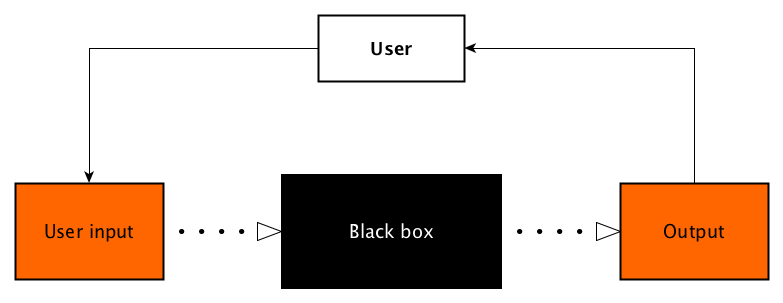
\includegraphics[scale=0.5]{./Fig/blackbox.png}
 \caption{Computational domain of the validation benchmark}
\end{figure}


Several commercial and  available solvers for FSI exists, both for monolithic and partitioned approaches. The commerical software ADINA makes solvers based on both approaches available for the user \cite{Zhang2003}. The open-source OpenFOAM also incoporate both solvers, howevere enabling more flexibillity in combining different solution strategies ... \\

The disiplines of CFD and computational structural dynamics (CSD) have tradidionally been treated separatly. Hence, highly optimized and specialized software has been developed individually, with little or no regard to multiphysics such as fluid-structure interaction.
Using a partitioned approach, the MpCCI interface is considered the "de-facto" software, for coupling separate fluid and solid solvers  [\cite{Wolf2007}, \cite{Geuzaine}].  \\

In this thesis a monolithic FSI-solver is developed without the use of commercial available software. The main motivation for this choice is the full understanding of the implementation, and the ability for code intervention along the solution process. The process of implementing a self-made solver for fluid-structure interaction is not stright forward. Due to the overall size of the total system,  and the assumption of a non-linear material and large deformations makes the process..

The implementation of the FSI-solver relies soley on the open-source project FEniCS, a computing platform for solving partial differential equation. The next section will present the general consepts for this.. 


\section{FEniCS}
The FEniCS project is an open-source finite element environment for solving partial differential equations (https://fenicsproject.org/). Using a combination of high-level Python and C++ interfaces, mathematical models can be implemented compactly and efficiently. FEniCS consists of several sub-modules and we will give a brief overview of the most central components used during implementation and computation.


\subsection{DOLFIN}
DOLFIN is the computational C++ backend of the FEniCS project, and the main user interface. It unifies several FEniCs components for implementing of computational mesh, function spaces, functions and finite element assembly. 

\begin{itemize} 
\item UFL (The Unified Form Language)  is a domain specific language, used for the discretization of mathematical abstractions of partial differential equations on a finite element form. Its implementation on top of Python, makes it excellent to define problems close to their mathematical notation without the use of more complex features. One uses the term \textit{form} to define any representation of some mathematical problem defined by UFL.   

\item FFC (The form compiler) compiles the finite elements variation forms given by UFL, generating low-level efficient C++ code 

\item FIAT the finite element backend, covering a wide range of finite element basis functions used in the discretization of of the  the finite-element forms. It covers a wide range of finite element basis functions for lines, triangles and tetrahedras.

\end{itemize}  


DOLFIN also incorporate the necessary interfaces to external linear algebra solvers and data structures. Within FEniCS terminology these are called linear algebra backends. PETSc is the default setting in FEniCS, a powerful linear algebra library
with a wide range of parallel linear and nonlinear solvers and efficient as matrix and vector operations for applications written in C, C++, Fortran and Python. \\
A comprehensive introduction FEniCS is out of the scope for this thesis, and for further insight the reader is directed to the introductional demos presented on https://fenicsproject.org/.  \\

\subsection{Poission Equation, hello world}
When learning programming, it is common to present a "Hello world!" program, presenting the fundamental concepts of the software of interest. For solving PDE's, one of the most basic challenges is solving the Possion's equation. Let $\Omega$ be the computational domain  and let $\partial \Omega$, be the boundary of $\Omega$. The Poission equation takes the form,
\begin{align*}
- \nabla^2 u = f \hspace{2mm} \in \Omega \\
u = u_d \hspace{2mm} \in \partial \Omega
\end{align*}
where u is the unknown of interest and f is some known function. $\nabla^2$ is the Laplace operator and $u = u_d$ is a prescribed Dirichlet condition on the boundary. 
Assuming the reader has some knowledge of the finite-element method, the unknown function u is approximated by a \textit{trial function}. The problem is then multiplied with a \textit{test function} v, and then we use integration by-parts over the domain $\Omega$. 

\begin{align*}
-\int_{\Omega} \nabla^2 u v dx = \int_{\Omega} f dx \\
- \int_{\partial \Omega} \frac{\partial u}{\partial n} v ds +
\int_{\Omega} \nabla u \nabla v dx = \int_{\Omega} f dx
\end{align*}
For simplicity, the \textit{test function} $v = 0$ on the boundary $\partial \Omega$ due to the prescribed Dirichlet condition which leaves us with the system

\begin{align*}
\int_{\Omega} \nabla u \nabla v dx = \int_{\Omega} f dx
\end{align*}

With the primilaries set, we focus on the implementation of the probelem in FEniCS. The poission problem can then be expressed,

\begin{python}[caption=posssion.py]
from fenics import *

# Create mesh and define a 1.order lagrangian function space
mesh = UnitSquareMesh(10, 10)
V = FunctionSpace(mesh, 'CG', 1)

# Define dirichlet boundary condition
u_bnd = Expression('1 + x[0]*x[0] + 2*x[1]*x[1]', degree=2)

bcs = DirichletBC(V, u_bnd, "on_boundary")

Define variational problem
u = TrialFunction(V)
v = TestFunction(V)
f = Constant(-10.0)
a = dot(grad(u), grad(v))*dx
L = f*v*dx

# Solve problem and compute solution
u = Function(V)
solve(a == L, u, bc)
\end{python}

The possion problem expressed with FEniCS points out two important properties. Frist, the overall problem is implemented compactly while each code segement for solving the problem remains clear.  Second, the abstract notation remains close to the orignal problem of interest. 

\section{implemented code}

The overall codestructure of the implementation is based on dividing the full code into fragments of Python modules. The main idea is to keep key code segments functionality while maintaining modularity to each code segment.

\begin{figure}[h!]
\hspace*{-2.2cm}
\centering    
 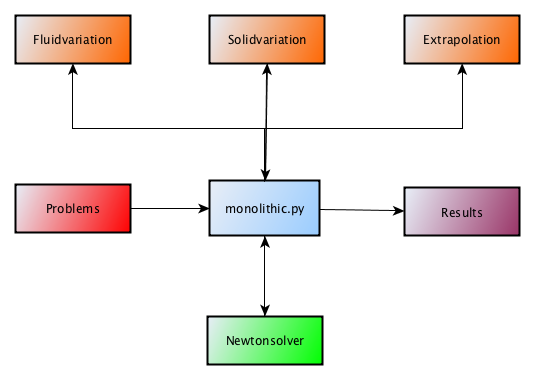
\includegraphics[scale=0.6]{./Fig/mapofsolver.png}
 \caption{Computational domain of the validation benchmark}
\end{figure}



 




  